\subsection{Bayes Filter}
The Bayes filter provides the probabilistic foundation for recursive state estimation. It describes how a systems state distribution evolves over time as new measurements are received, based on the principles of Bayesian inference. The filter assumes that the process and measurement models form a Markov chain, where the current state $\mathbf{x}_k$ depends only on the previous state $\mathbf{x}_{k-1}$ and control input $\mathbf{u}_{k-1}$, and each measurement $\mathbf{z}_k$ depends only on the current state.  
\\ \\
This structure is known as a Hidden Markov Model, where the underlying system state is hidden and only indirectly observed through noisy sensor measurements. The process and measurement noise are assumed to be white, zero mean, and statistically independent, ensuring that all uncertainty can be modeled probabilistically within the Bayesian framework.  
\\ \\
The Bayes filter operates recursively in two stages: prediction and update. The \textit{``prediction step''} propagates the previous state estimate forward in time using the process model:
$$
    p(\mathbf{x}_k | \mathbf{z}_{1:k-1}) = \int p(\mathbf{x}_k | \mathbf{x}_{k-1})\,p(\mathbf{x}_{k-1} | \mathbf{z}_{1:k-1})\,d\mathbf{x}_{k-1}
$$
This step accounts for system dynamics and process noise, providing a prior belief of the current state before any new measurement is considered.  
\\ \\
The \textit{``update step''} then incorporates the new measurement $\mathbf{z}_k$ to refine the estimate:
$$
    p(\mathbf{x}_k | \mathbf{z}_{1:k}) =
    \frac{p(\mathbf{z}_k | \mathbf{x}_k)\,p(\mathbf{x}_k | \mathbf{z}_{1:k-1})}
    {\int p(\mathbf{z}_k | \mathbf{x}_k)\,p(\mathbf{x}_k | \mathbf{z}_{1:k-1})\,d\mathbf{x}_k}
$$
Here, the numerator represents the likelihood of observing the measurement given a state hypothesis, multiplied by the predicted prior, while the denominator ensures normalization of the resulting probability distribution.  
\\ \\
This recursive formulation captures the fundamental idea of probabilistic state estimation, where one combines prior knowledge with new information to obtain a posterior estimate. In practice, however, exact computation of these integrals is rarely feasible due to nonlinear process models, non Gaussian noise, and the high dimensionality of the state space. Evaluating the full probability distributions quickly becomes computationally intractable for real-time systems.  
\\ \\
For this reason, practical implementations rely on approximate Bayesian filters that make simplifying assumptions to achieve tractable computation. The Kalman Filter assumes linear models with Gaussian noise, while the Extended Kalman Filter and Unscented Kalman Filter extend these ideas to nonlinear systems using local linearization or deterministic sampling. These methods retain the core Bayesian structure but operate with compact parametric representations of uncertainty, typically through the state mean and covariance.  
\\ \\
A simplified overview of the process and measurement relationships is shown in Figure \ref{fig:state-estimation-hidden-markov-model}. The figure illustrates how control inputs $\mathbf{u}_k$ influence the system state $\mathbf{x}_k$, which in turn generates measurements $\mathbf{z}_k$ through a noisy observation model.  
\\ \\
The formulation and structure presented here follow the conventions introduced by Edmund Brekke in \textit{``Fundamentals of Sensor Fusion''} \cite{sensor_fusion_book}, which form the theoretical foundation for the estimation framework implemented in this thesis.
\begin{figure}[H]
    \centering
    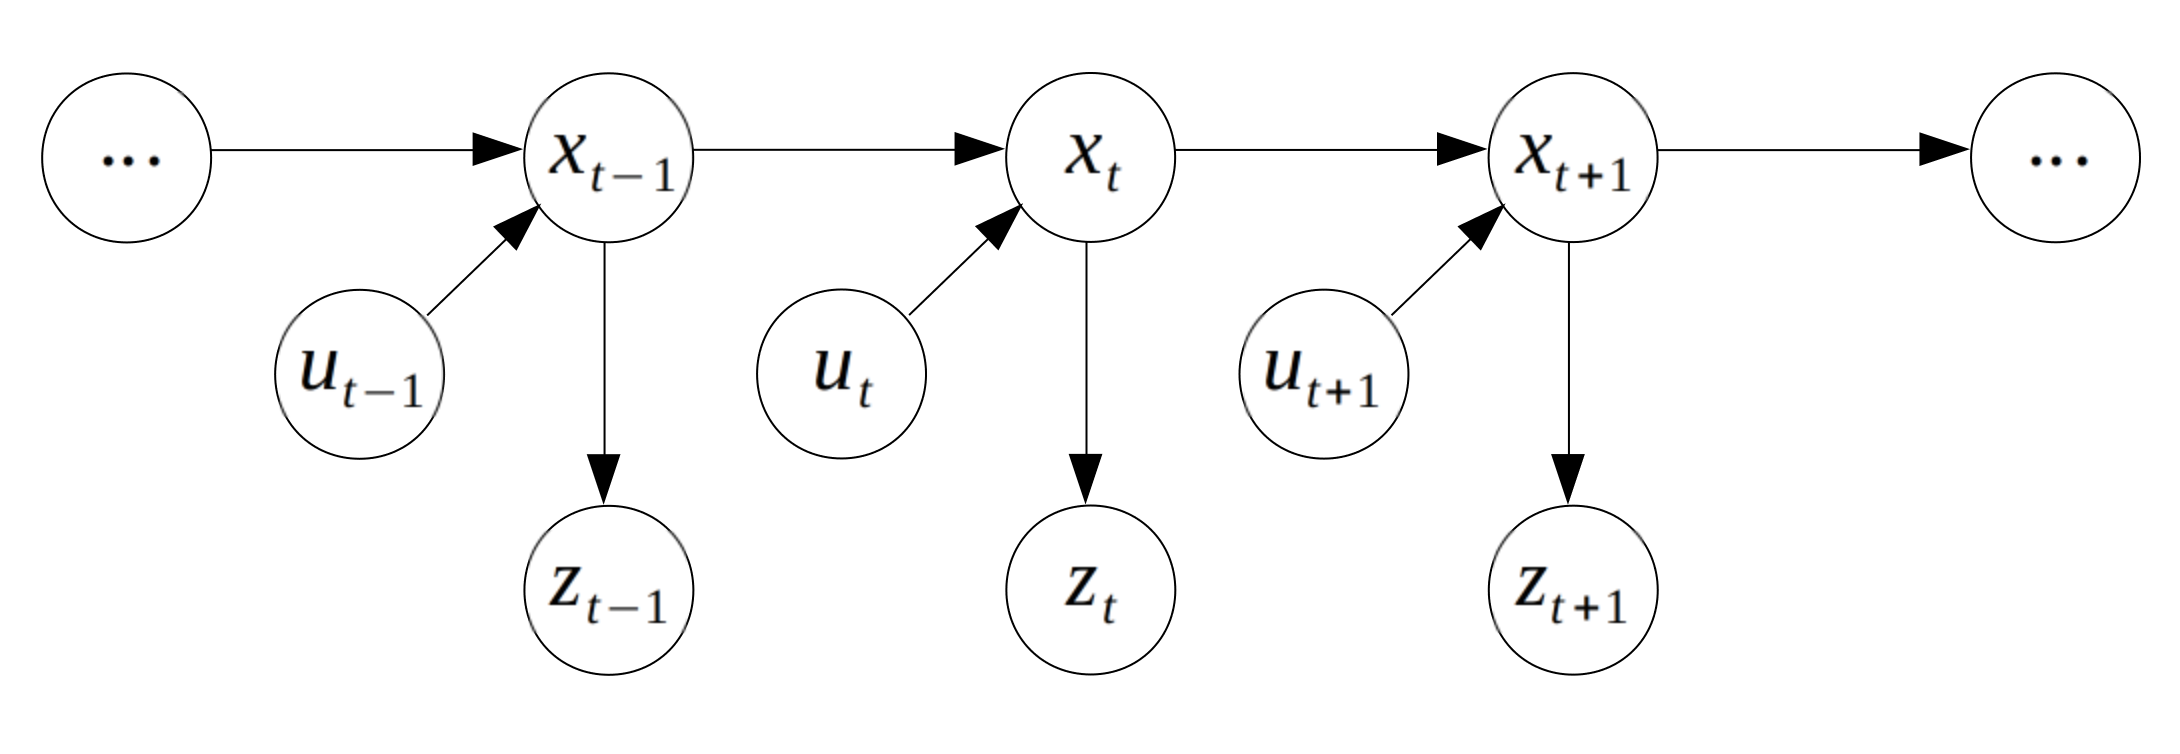
\includegraphics[width=1.0\linewidth]{Pictures/State_Estimation/Bayes_Filter/Hidden_Markov_Model.png}
    \caption{Hidden Markov Model representation of the Bayes filter, showing the relationships between state $\mathbf{x}$, measurement $\mathbf{z}$, and control input $\mathbf{u}$. Image sourced from Lei Mao blog on Bayes Filters.\textsuperscript{\cite{bayes_filter}}}
    \label{fig:state-estimation-hidden-markov-model}
\end{figure}

